\documentclass[11pt]{article}
\usepackage{graphicx}
\usepackage{minted}
\setminted[xml]{fontsize=\footnotesize}
\setmintedinline[xml]{fontsize=\normalsize}
\usepackage{bookmark,hyperref}
\hypersetup{
    colorlinks=true,
    linkcolor=blue,
    citecolor=blue,
}

\newcommand{\xfouri}{\texttt{x4i}}

\begin{document}

\title{\xfouri, The EXFOR interface}
\author{David A. Brown\footnote{Point of contact, email \url{dbrown@bnl.gov}}\ \footnote{National Nuclear Data Center, Brookhaven National Laboratory, Upton, NY 11973} \ and Grier Sayers\footnote{Department of Geology and Physics, Lock Haven University of Pennsylvania, Lock Haven, PA 17745}}
\date{7 August 2019}
\maketitle
\begin{center}
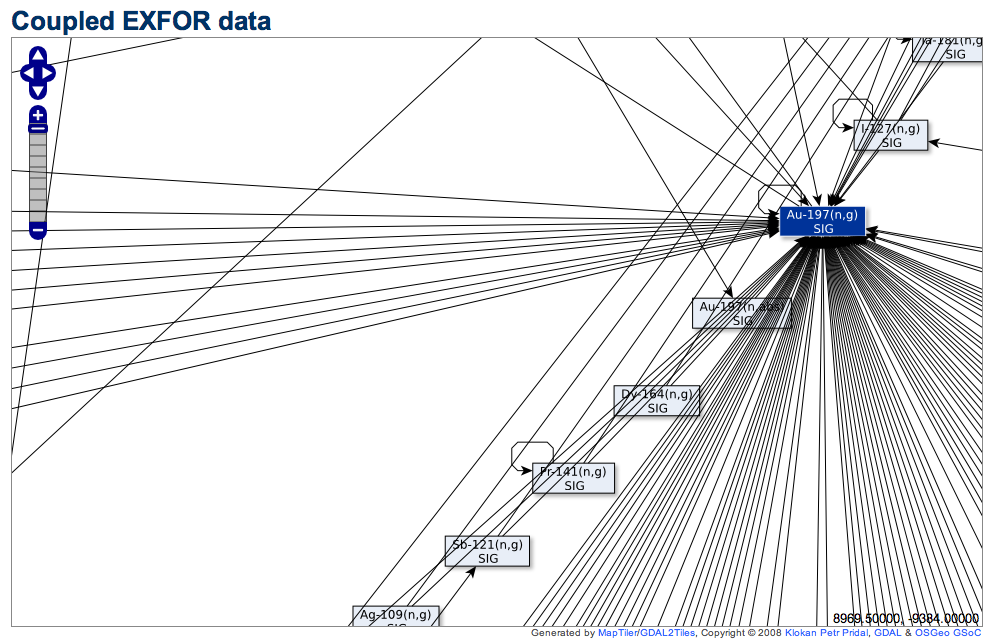
\includegraphics[width=0.8\textwidth]{figs/vis.png}
\end{center}

\tableofcontents

\section{Introduction}
The \xfouri\ package is an interface to the EXFOR nuclear data library.  It simplifies retrieval of EXFOR entries and can automatically parse them, allowing one to extract cross-section (and other) data in a simple, plot-able format.  \xfouri\ also understands and can parse the entire reaction string, allowing one to build a strategy for processing the data.

EXFOR is a structured markup language for representing measured nuclear data.  It is an old format, and is awkward to use for several reasons:\begin{itemize}
\item  It relies on data being in the correct columns in order to denote context.  This is a legacy feature since EXFOR data used to be stored on FORTRAN punch cards.
\item The data was often hand entered so the format rules were not always rigorously obeyed (fortunately WPEC SubGroup 30 has remedied much of this ensuring that EXFOR data can  be translated into C4 format, see ref. \cite{1}).
\item The mark-up language is surprisingly complex (see refs. \cite{2,3,4,5}]).   Figures 1-5 illustrate the structure of the EXFOR format.
\end{itemize}

\begin{figure}[htbp]
\begin{center}
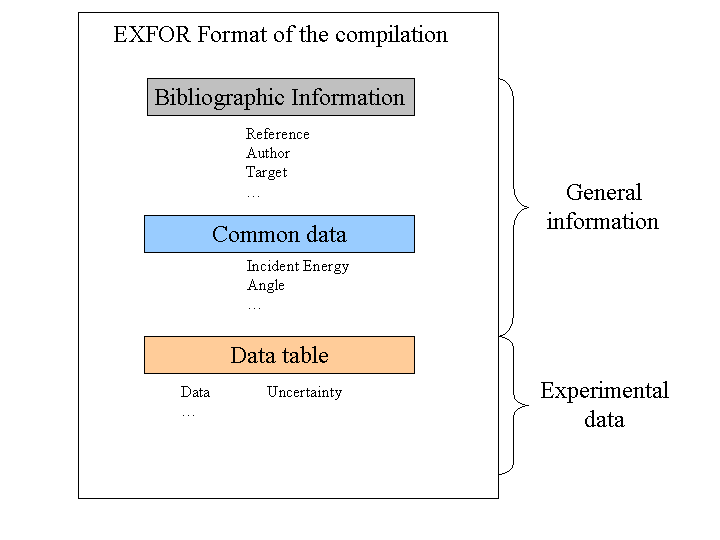
\includegraphics[width=0.7\textwidth]{figs/exfor02.png}
\caption{\label{fig:1}Structure of an EXFOR entry.  The bibliographic information is always contained in the first subentry of an entry and given the index `001'.  Common data is data common to all data blocks in all subentries and is found in the `001' subentry.  Each dataset is given its own subentry, beginning with subentry `002.'  Figure from ref. \cite{web}.}
\end{center}
\end{figure}

\begin{figure}[htbp]
\begin{center}
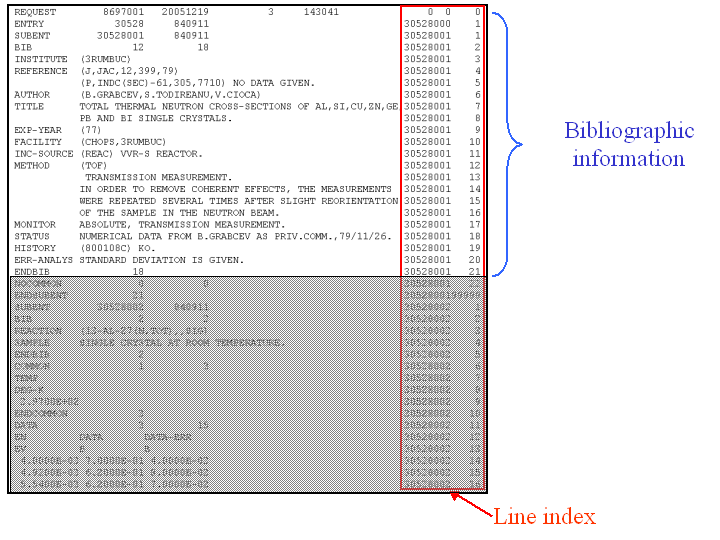
\includegraphics[width=0.7\textwidth]{figs/bib01.png}
\caption{\label{fig:2}A close-up on the first subentry showing the bibliographic data.  Figure from ref. \cite{web}.}
\end{center}
\end{figure}

\begin{figure}[htbp]
\begin{center}
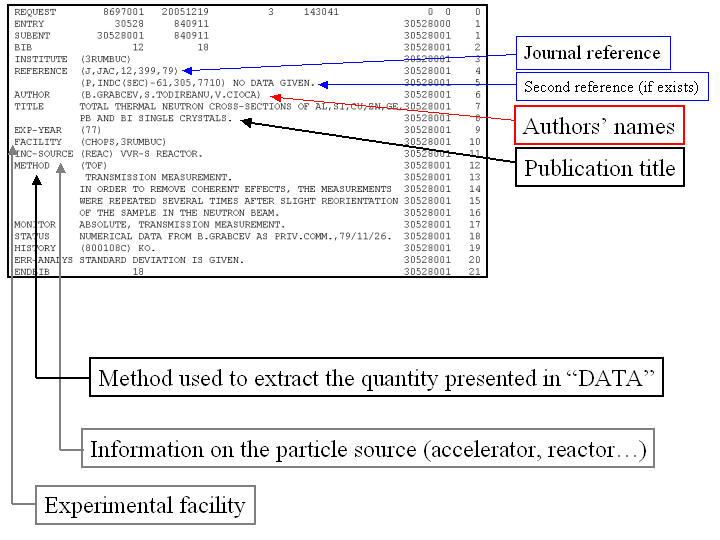
\includegraphics[width=0.7\textwidth]{figs/bib02.png}
\caption{\label{fig:3}An even closer look at the details of the bibliographic data.  Here one can see how the authors' names, institutions and publication information are specified.  Figure from ref. \cite{web}.}
\end{center}
\end{figure}

\begin{figure}[htbp]
\begin{center}
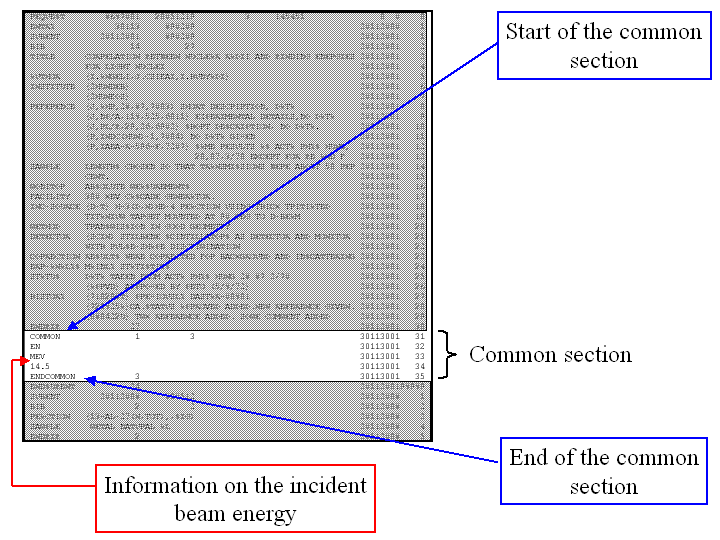
\includegraphics[width=0.7\textwidth]{figs/bib03.png}
\caption{\label{fig:4}A sample COMMON data section.  In this case, the beam energy for all data in subsequent subentries is given.  Figure from ref. \cite{web}.}
\end{center}
\end{figure}

\begin{figure}[htbp]
\begin{center}
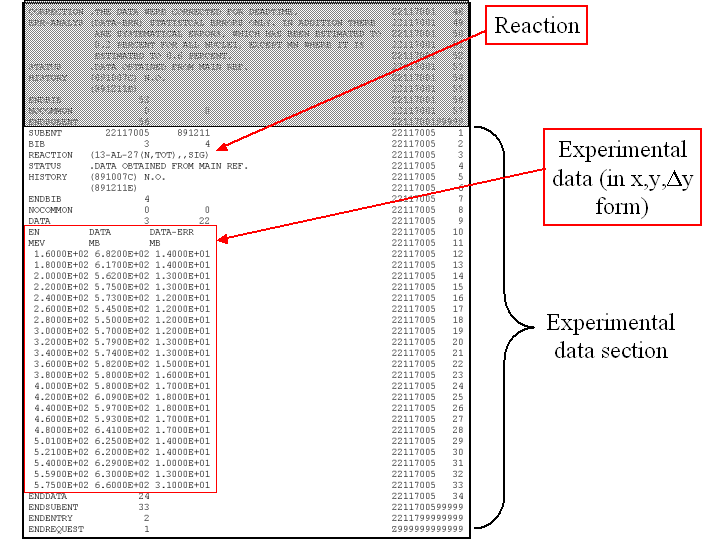
\includegraphics[width=0.7\textwidth]{figs/bib04.png}
\caption{\label{fig:5}A sample DATA section.  DATA sections contain the actual data from a measurement.   This is combined with the data in COMMON data to produce an instance of the \texttt{X4DataSet} class detailed later in this report.  Figure from ref. \cite{web}.}
\end{center}
\end{figure}

\clearpage

\section{Installation}
There are several ways to install \xfouri.  They are given below in order of increasing difficulty.
Please ensure your `git` installation has large file support (see https://git-lfs.github.com).

\subsection{Easiest installation: using pip and git}
\begin{minted}[frame=single,fontsize=\small]{sh}
host$ pip install git+https://github.com/brown170/x4i
\end{minted}
This version of the installation process automatically installs the 2021-03-08 version of the EXFOR database.

\subsection{Installation from a tarball distribution}

\begin{enumerate}
\item Unpack the distribution

\item Installation options:
  \begin{itemize}
  \item Old-fashioned local installation: put \xfouri\ in your \texttt{\$PYTHONPATH}.  Assuming you are in the directory containing \xfouri's `setup.py` file:
    \begin{minted}[frame=single,fontsize=\small]{sh}
      host$ export PYTHONPATH=$PYTHONPATH:\`pwd\`
    \end{minted}

  \item Installation with pip (You can delete the \xfouri\ project once this is complete)
    \begin{minted}[frame=single,fontsize=\small]{sh}
      host$ pip install path/to/x4i/setup.py/directory
    \end{minted}

  \item Editable pip installation
    \begin{minted}[frame=single,fontsize=\small]{sh}
      host$ pip install -e path/to/x4i/setup.py/directory
    \end{minted}

  \item For site-wide installation.  Assuming you are in the directory containing \xfouri's \texttt{setup.py} file (You can delete the \xfouri\ project once this is complete):
    \begin{minted}[frame=single,fontsize=\small]{sh}
    host$ sudo python setup.py install
    \end{minted}

  \end{itemize}

\end{enumerate}

\subsection{Source installation from git}

This assumes that you will be editing the project in some fashion.
This installation does not automatically include the IAEA data files.
You will need to download them yourself as described in step \#3. below.

\begin{enumerate}
\item Clone the project
\begin{minted}[frame=single,fontsize=\small]{sh}
host$ git clone https://github.com/brown170/x4i.git
\end{minted}

\item Installation options:
  \begin{itemize}
    \item Old-fashioned local installation: put \xfouri\ in your \texttt{\$PYTHONPATH}.  Assuming you are in the directory containing \xfouri's \texttt{setup.py} file:
      \begin{minted}[frame=single,fontsize=\small]{sh}
      host$ export PYTHONPATH=$PYTHONPATH:\`pwd\`
      \end{minted}

    \item Editable installation using pip:
      \begin{minted}[frame=single,fontsize=\small]{sh}
      host$ pip install -e path/to/x4i/setup.py/directory
      \end{minted}
  \end{itemize}

\item To get the EXFOR library from the IAEA, run the install script.  This will install the 2021-03-08 version.  Assuming you are in the directory containing \xfouri's \texttt{setup.py} file, do:
  \begin{minted}[frame=single,fontsize=\small]{sh}
   host$ ./install.py
  \end{minted}
\end{enumerate}


\section{Upgrading}
To update or change the source database, you will need a copy of the new database from the IAEA.  It is available as a zipfile downloaded from the IAEA website: \url{http://www-nds.iaea.org/x4toc4-master/.}  There are two sets of files there.  Those with the name of the form \texttt{X4-YYYY-MM-DD.zip} are the ones usable by \xfouri.  To install the IAEA library, assuming that your zip file is named  \texttt{X4-YYYY-MM-DD.zip}:
\begin{minted}[frame=single,fontsize=\footnotesize]{sh}
$host python bin/setup-exfor-db.py --x4c4-master ~/Downloads/X4-2019-07-18.zip
13535: (1991) A.Ling, X.Aslanoglou, et al.
13564: (1970) J.Taylor, G.Spalek, et al.
13597: (1995) S.K.Ghorai, P.M.Sylva, et al.
13550: (1992) C.M.Castaneda, R.Gearhart, et al.
13501: (1991) R.R.Winters, R.F.Carlton, et al.
13511: (1991) C.M.Perey, F.G.Perey, et al.
13540: (1989) S.Nath, G.Glass, et al.
13587: (1993) R.Macklin, N.W.Hill, et al.
...
\end{minted}
Please read the help message (\texttt{python bin/setup-exfor-db.py -h}) for more information.  After you finish this step,
be sure to update the information in the \texttt{x4i/data/database\_info.json} file.

\section{Basic Usage}
Now we describe how to use \xfouri.  We begin by explaining how to query the EXFOR database and how to retrieve data.  All retrievals and queries are handled by the classes in the \texttt{exfor\_manager} module.  The class \texttt{X4DBManagerDefault} defaults to the \texttt{X4DBManagerPlainFS} class and this is the class supported out of the box by \xfouri.  Here is an example of its use:
\begin{minted}[frame=single,fontsize=\footnotesize]{pycon}
Python 3.7.3 (default, Mar 30 2019, 03:37:43)
[Clang 10.0.0 (clang-1000.11.45.5)] on darwin
Type "help", "copyright", "credits" or "license" for more information.
>>> from x4i import exfor_manager
>>> db = exfor_manager.X4DBManagerDefault()
>>> help(db)
Help on X4DBManagerPlainFS in module x4i.exfor_manager object:

class X4DBManagerPlainFS(X4DBManager)
 |  X4DBManagerPlainFS(**kw)
 |
 |  EXFOR data base manager for data stored on local filesystem in
 |  directory hierarchy.
 |
 |  Method resolution order:
 |      X4DBManagerPlainFS
 |      X4DBManager
 |      builtins.object
 |
 |  Methods defined here:
 |
 |  __init__(self, **kw)
 |      Initialize self.  See help(type(self)) for accurate signature.
 |
 |  query(self, author=None, reaction=None, target=None, projectile=None,
 |        quantity=None, product=None, MF=None, MT=None, C=None, S=None,
 |        I=None, SUBENT=None, ENTRY=None, reference=None)
 |      Use this function to search for all (Sub)Entries matching
 |      criteria in query call.  This function returns a dictionary
 |      with the following structure::
 |
 |         { ENTRY:[ SUBENT001, SUBENT002, SUBENT003, ... ], ... }.
 |
 |      Here ENTRY is the entry number whose subentries match the query.
 |      The SUBENT001 is the documentation subentry number, which is
 |      always included, and SUBENT002, ... are the subentry numbers
 |      matching the search criteria.
 |
 |  retrieve(self, author=None, reaction=None, target=None,
 |           projectile=None, quantity=None, product=None, MF=None,
 |           MT=None, C=None, S=None, I=None, SUBENT=None,
 |           ENTRY=None, rawEntry=False, reference=None)
 |      Execute a query, matching the criteria specified.
 |      This function returns a dictionary with the following
 |      structure::
 |
 |          { ENTRY:[ SUBENT001, SUBENT002, SUBENT003, ... ], ... }.
 |
 |      Here ENTRY is the entry number whose subentries match the
 |      query.  The SUBENT001 is the documentation subentry itself,
 |      which is always included, and SUBENT002, ... are the
 |      subentries themselves matching the search criteria.
 |
 |      If the flag rawEntry is True, the raw text versions of the
 |      SUBENTs will be returned, otherwise they will be converted
 |      to X4Entry instances.
...
\end{minted}
Once the database manager is initialized, we can run a query:
\begin{minted}[frame=single,fontsize=\small]{pycon}
>>> db.query(author='Panitkin')
{'40121': ['40121001', '40121002'], '40177': ['40177001',
'40177002', '40177003'], '41335': ['41335001', '41335002'],
'41654': ['41654001', '41654002']}
\end{minted}
All queries return a Python \texttt{dict}.  The keys of the dictionary are the EXFOR entry number.  The values of the dictionary are a list of subentry numbers of the EXFOR entry whose contents match the query search criteria.  If a particular subentry matches the search criteria, the corresponding documentation subentry  (the `001' subentry) is also returned.  The complete list of search criteria  are given in Table \ref{table:search}.  A partial list of searchable observables is given in Table \ref{table:observables}.

\begin{table}
\caption{Valid search keys for queries and retrievals from the EXFOR database manager classes.  One key not mentioned in this table is the recently added \texttt{reference} key.}
\begin{center}
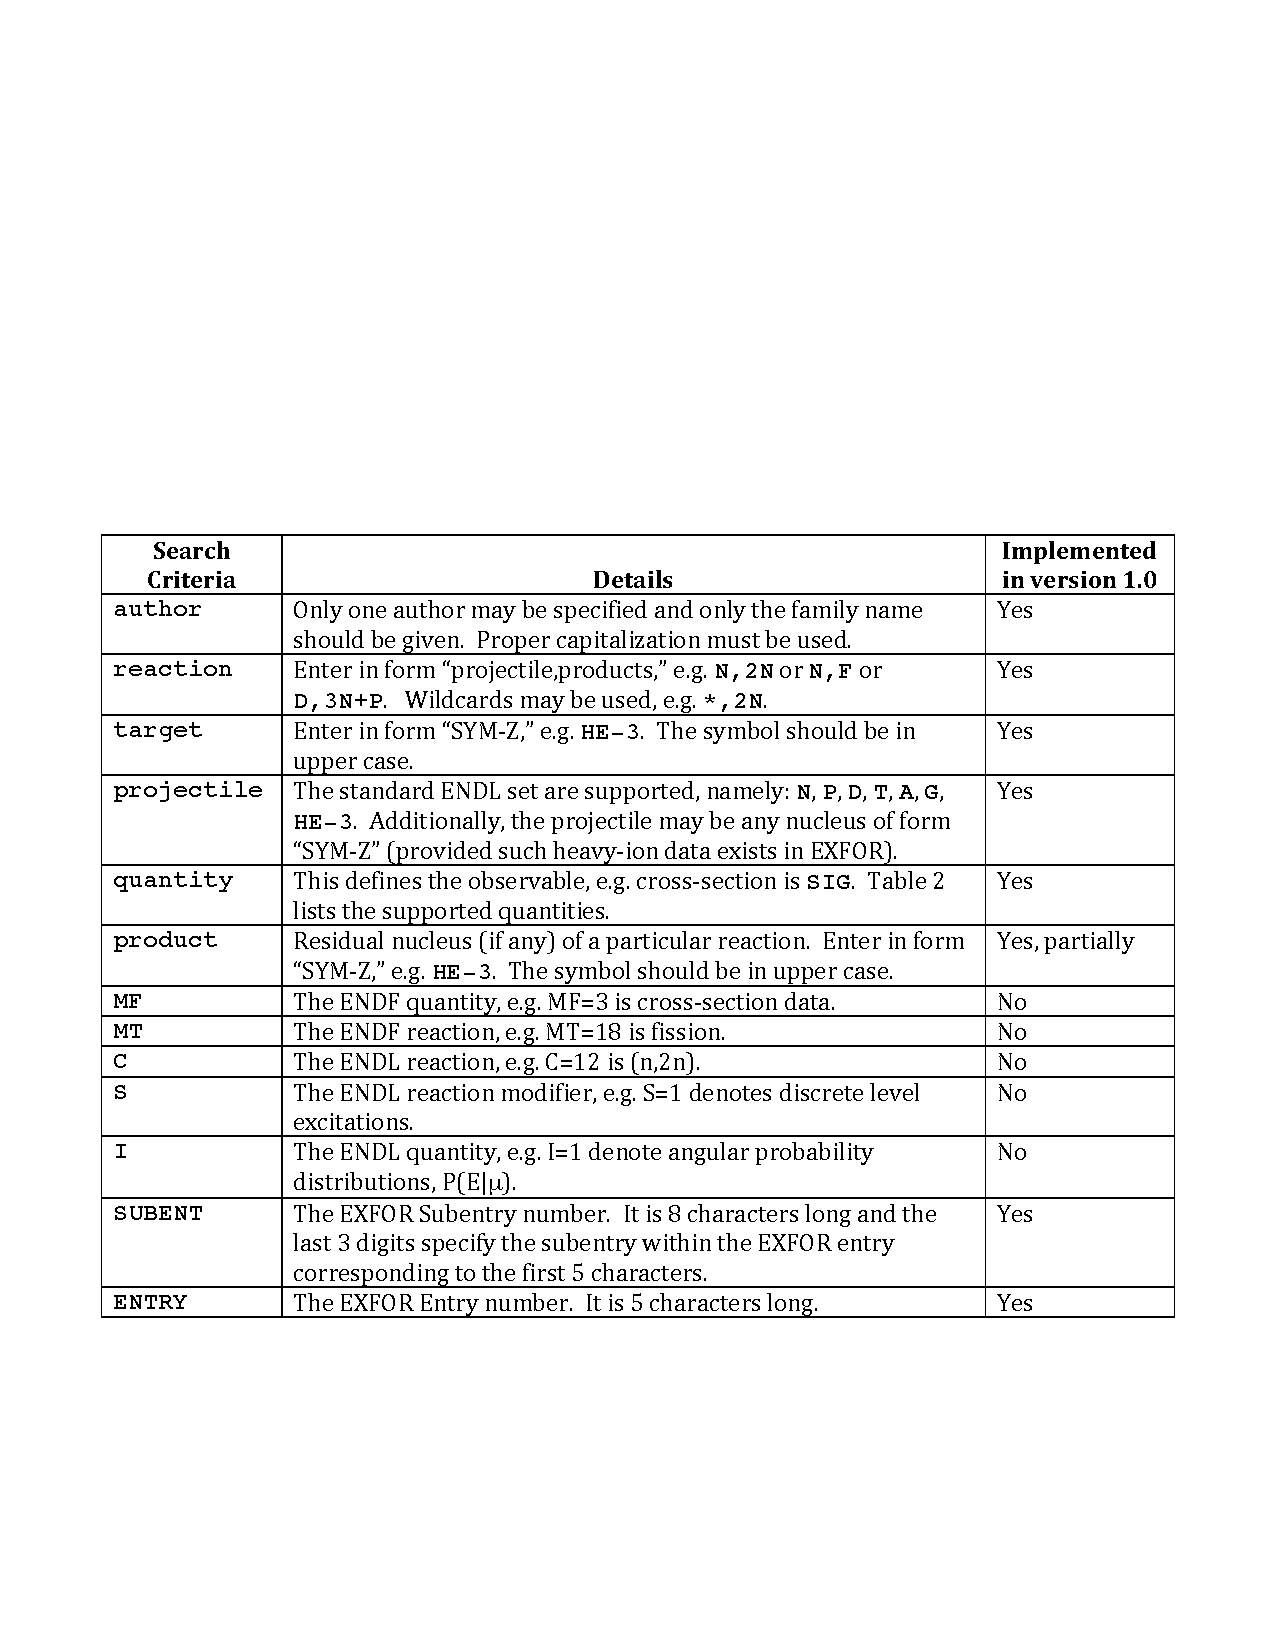
\includegraphics[width=0.9\textwidth]{tables/table1}
\end{center}
\label{table:search}
\end{table}%

\begin{table}
\caption{A selection of supported quantities.  The full list is given in EXFOR dictionary 30 (see ref. \cite{3})}
\begin{center}
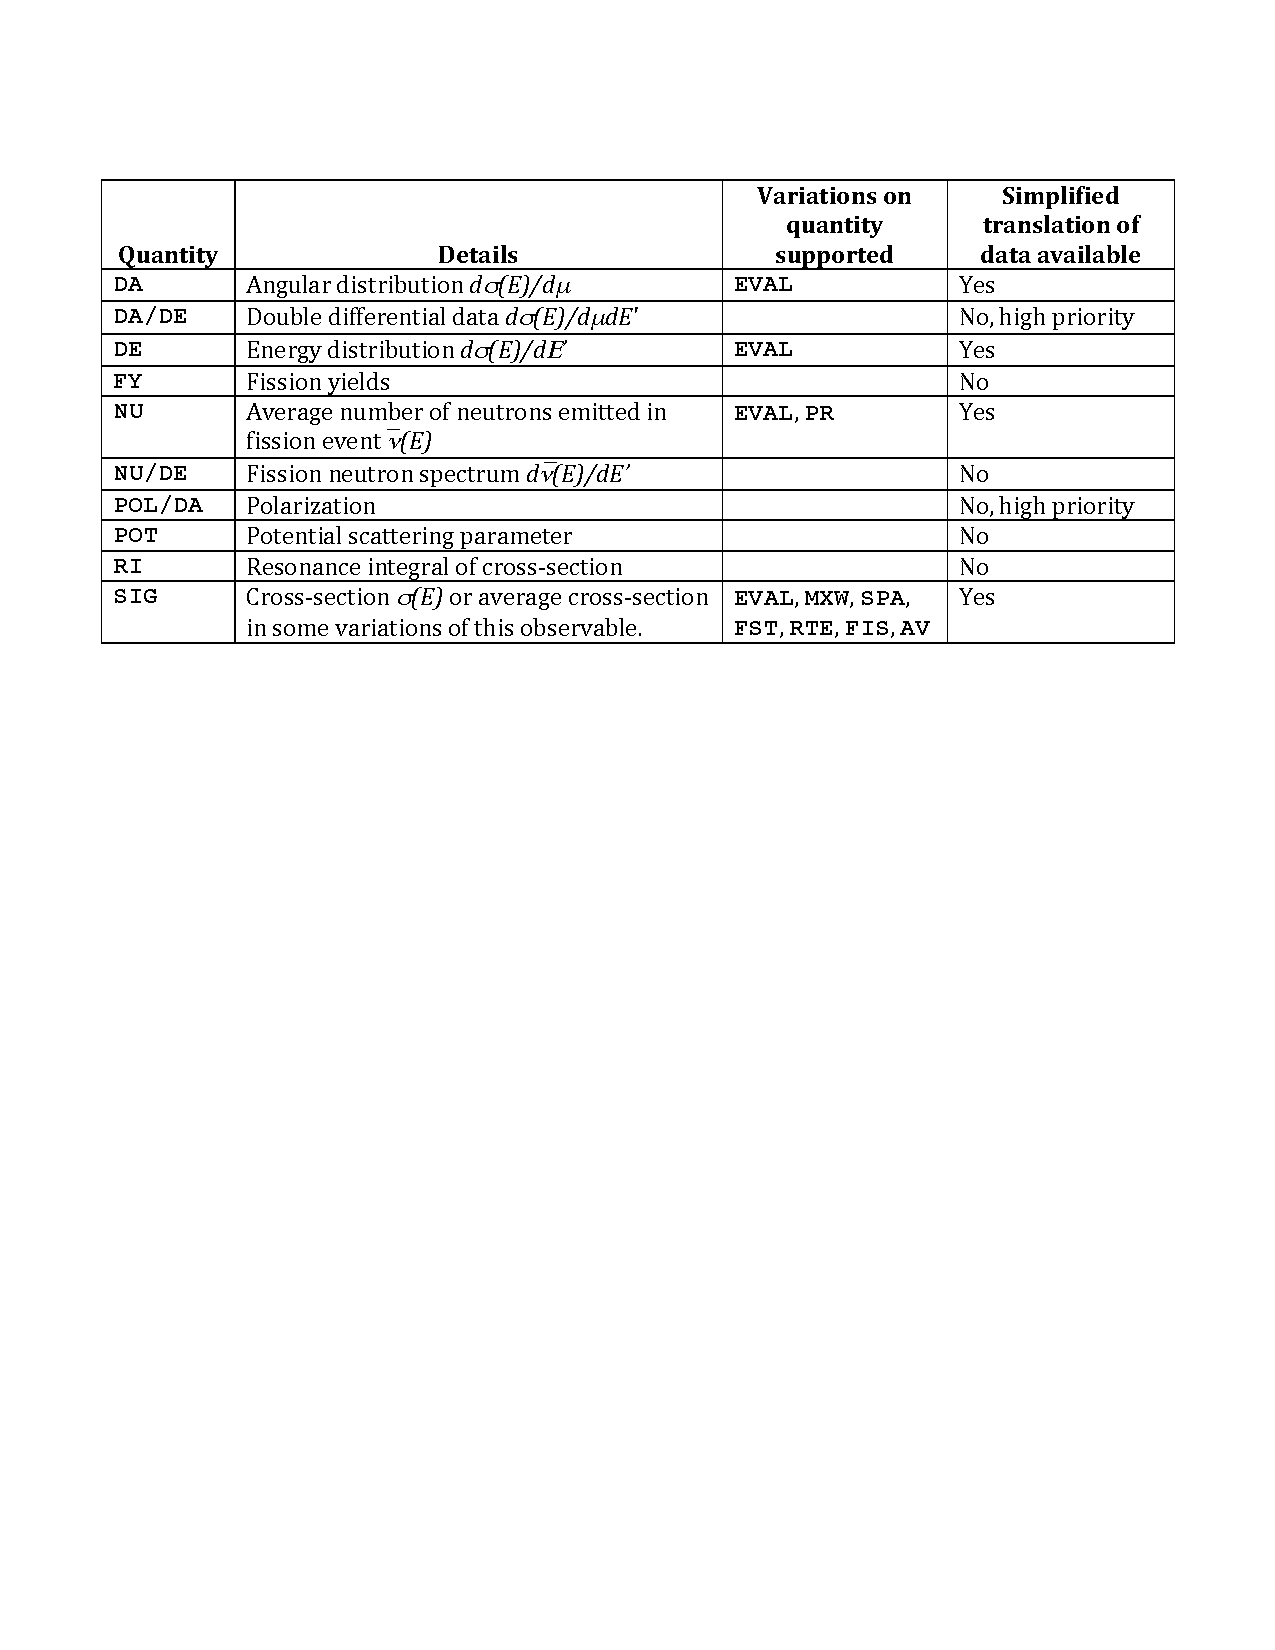
\includegraphics[width=0.9\textwidth]{tables/table2}
\end{center}
\label{table:observables}
\end{table}%


Retrievals also can be made using the database manager:
\begin{minted}[frame=single,fontsize=\small]{python}
>>> r=db.retrieve(author='Panitkin')
\end{minted}
The search result from a retrieval is a Python \texttt{dict}.  The keys are the ENTRY number (as a string) and the values are \texttt{X4Entry} instances:
\begin{minted}[frame=single,fontsize=\small]{pycon}
>>> for k in r:
...  print(k)
...
40121
40177
41335
41654
>>> type(r[40121])
Traceback (most recent call last):
  File "<stdin>", line 1, in <module>
KeyError: 40121
>>> type(r['40121'])
<class 'x4i.exfor_entry.X4Entry'>
\end{minted}
The \texttt{X4Entry} class is a member of the \texttt{exfor\_entry} module and handles all of the parsing of an EXFOR ENTRY.

In the following section, we will detail some of the things one can do with an \texttt{X4Entry} instance.  For now, we'll just illustrate hoe to extract the cross-section data in a format we can plot:
\begin{minted}[frame=single,fontsize=\small]{pycon}
>>> x=db.retrieve(target="PU-239", reaction="N,2N", quantity="SIG")
>>> x.keys()
dict_keys(['13787', '14129', '20795', '21971'])
>>> x['14129']
ENTRY      14129
SUBENT     14129001
BIB                 12         20
INSTITUTE  (1USALAS,1USALRL)
REFERENCE  (J,NSTS,2,(1),620,2002)
AUTHOR     (J.A.Becker,L.A.Bernstein,W.Younes,D.P.McNabb,
            P.E.Garrett,D.E.Archer,C.A.McGrath,M.A.Stoyer,H.Chen,
...
>>> y=x['14129']
>>> dss=y.getSimplifiedDataSets()
>>> dss.keys()
dict_keys([('14129', '14129002', ' ')])
>>> print(dss[('14129', '14129002', ' ')])
#  Authors:   J.A.Becker, L.A.Bernstein, W.Younes, D.P.Mcnabb, ...
#  Title:     Partial Gamma-Ray Cross Sections For The Reaction ...
#  Year:      2002
#  Institute: Lawrence Livermore National Laboratory, Livermore, CA
#  Reference: J.Nucl.Science and Technol.Tokyo,Supplement 2, ...
#  Subent:    14129002
#  Reaction:  Cross section for 239Pu(n,2n)238Pu
#        Energy        Data          d(Energy)     d(Data)
#        MeV           barns         MeV           barns
        6.481         0.1009        0.2239        0.03081
...
\end{minted}
What we've done here is extract all the datasets in our \texttt{X4Entry}  instance using the \texttt{getSimplifiedDataSets()} member function.  The results are stored in another Python \texttt{dict}, this time keyed off with a Python \texttt{tuple} with the following structure: \texttt{(entry \#, subentry \#, pointer)}.  In this case, there is no pointer  so that spot is taken by a string comprising a single space character.   In other cases, the pointer may be number either referring to additional data.  We will explain this further in the next sections.

\section{Main Classes}

\subsection{The \texttt{X4Entry} class}

In this section,  we provide a more detailed look into the \texttt{X4Entry} class and its use.  A partial list of member functions is provided in Table \ref{table:x4entry}.

Let us begin the discussion by picking up where we left off in the previous section's example.  We return to the \texttt{X4Entry} in the Python variable `y':
\begin{minted}[frame=single,fontsize=\small]{pycon}
>>> y=x['14129']
>>> y.keys()
dict_keys(['14129001', '14129002'])
>>> type(y[1])
<class 'x4i.exfor_subentry.X4SubEntry'>
\end{minted}
In this simple example, we have illustrated that \texttt{X4Entry}s are really Python \texttt{dict}s, with keys  being the subentry accession number (in this case, abbreviated to `1') and values being instances of the \texttt{X4SubEntry} class.  Note that the subentry accession numbers 1, `1', `001', 13883001, and `1388301' are all equivalent.   Continuing:
\begin{minted}[frame=single,fontsize=\small]{pycon}
>>> y['1'].keys()
dict_keys(['BIB'])
>>> y['1']['BIB'].keys()
dict_keys(['INSTITUTE', 'REFERENCE', 'AUTHOR', 'TITLE', 'FACILITY',
           'INC-SPECT', 'DETECTOR', 'SAMPLE', 'METHOD', 'ANALYSIS',
           'MONITOR', 'HISTORY'])
>>> y['1']['BIB']['REFERENCE'].keys()
dict_keys([' '])
>>> y['1']['BIB']['REFERENCE'][' ']
           (J,NSTS,2,(1),620,2002)
>>> str(y['1']['BIB']['REFERENCE'][' '])
'(J,NSTS,2,(1),620,2002)'
\end{minted}
Clearly \texttt{X4Entry}s and \texttt{X4SubEntry}s are simply nested Python \texttt{dict}s whose keys and values  correspond to the structure of the original EXFOR (sub)entry.  This example illustrates one other point:  the Python \texttt{str()} operator returns a ``pretty'' version of what it acts on.  In this case, the reference field of the bibliography section of subentry \#1.

There are two other functions to elaborate, the \texttt{getSimplifiedDataSets()} and \texttt{getDataSets()} function.  Both return \texttt{dict}s whose values are \texttt{X4DataSets}, either ``plain'' or ``simplified.''  In the next section we will describe the \texttt{X4DataSet} and explain the difference between a ``plain'' \texttt{X4DataSet} and a ``simplified'' \texttt{X4DataSet}.  Here we illustrate the use of either function:
\begin{minted}[frame=single,fontsize=\small]{pycon}
>>> dss = y.getSimplifiedDataSets()
>>> dss.keys()
dict_keys([('14129', '14129002', ' ')])
\end{minted}
This function returns a Python dict whose keys are a tuple:  \texttt{(entry \#, subentry \#, pointer)}.  The EXFOR pointer here is a string consisting of a space.  In many EXFOR subentries, the EXFOR compilers chose to store multiple datasets.  To distinguish them (and to map the data  to other fields in the EXFOR entry), the compilers gave the sets a distinct one character pointer.  When \xfouri\ encounters such a case, the dict returned from \texttt{getSimplifiedDataSets()} will have one key per pointer.

\begin{table}
\caption{Member function reference for the \texttt{X4Entry} class and the \texttt{X4EntryMetaData} class. Functions in the \texttt{X4EntryMetaData} class are prefixed with the \texttt{meta()} call from the \texttt{X4Entry} class.}
\begin{center}
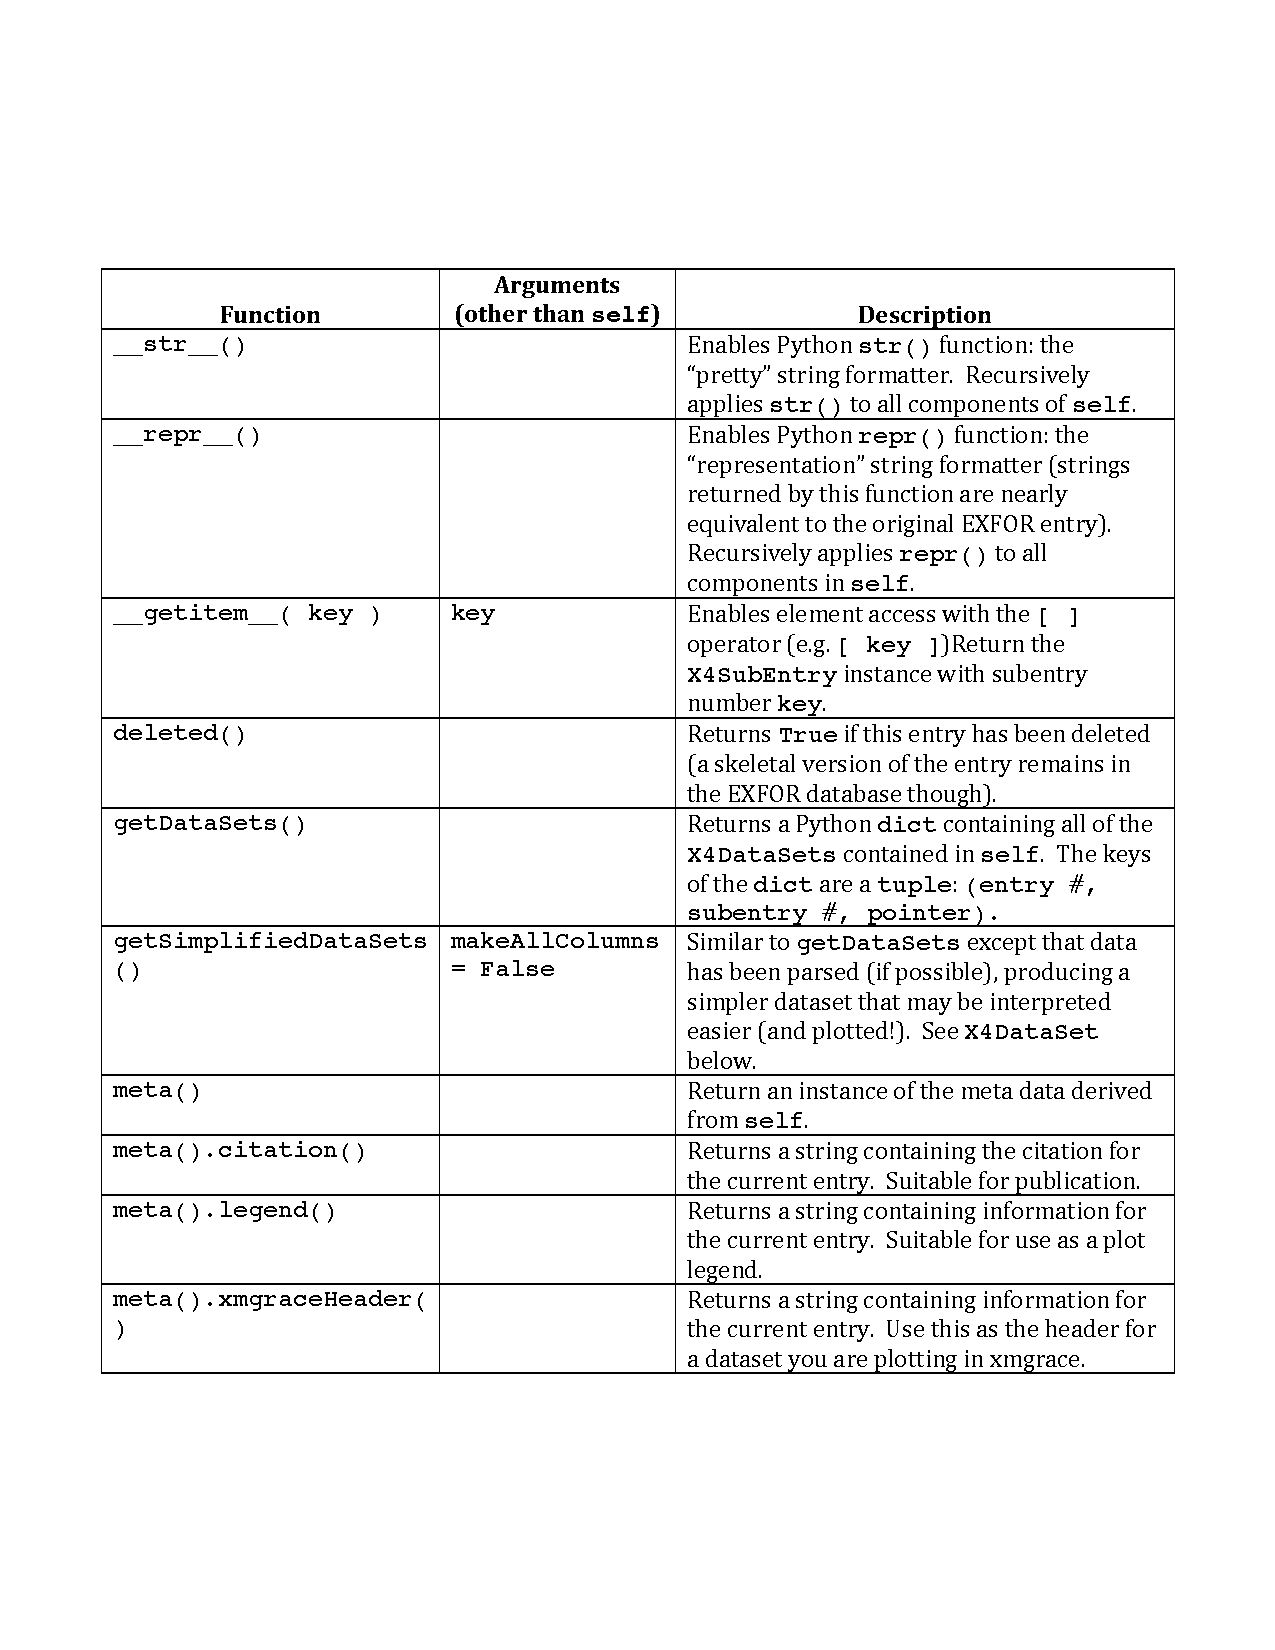
\includegraphics[width=0.9\textwidth]{tables/table3}
\end{center}
\label{tabels:x4entry}
\end{table}%


\subsection{The \texttt{X4DataSet} class}

The \texttt{X4DataSet} class and its subclasses are probably the class most users of \xfouri\ will become familiar with first as instances of these classes contain the experimental data one wishes to plot and/or manipulate.  In the previous section we introduced two functions in the \texttt{X4Entry} class that return \texttt{dict}s containing \texttt{X4DataSet}s.  We also introduced the concept of ``plain'' and ``simplified'' datasets.  Figure \ref{fig:6} shows the \texttt{csv} output of the \texttt{X4DataSet}, retrieved in the previous section, in its ``plain'' form and its ``simplified'' form.  As one can see, both contain the same data, but the ``simplified'' set is in consistent units and extraneous columns have been removed.

\begin{figure}[htbp]
\begin{center}
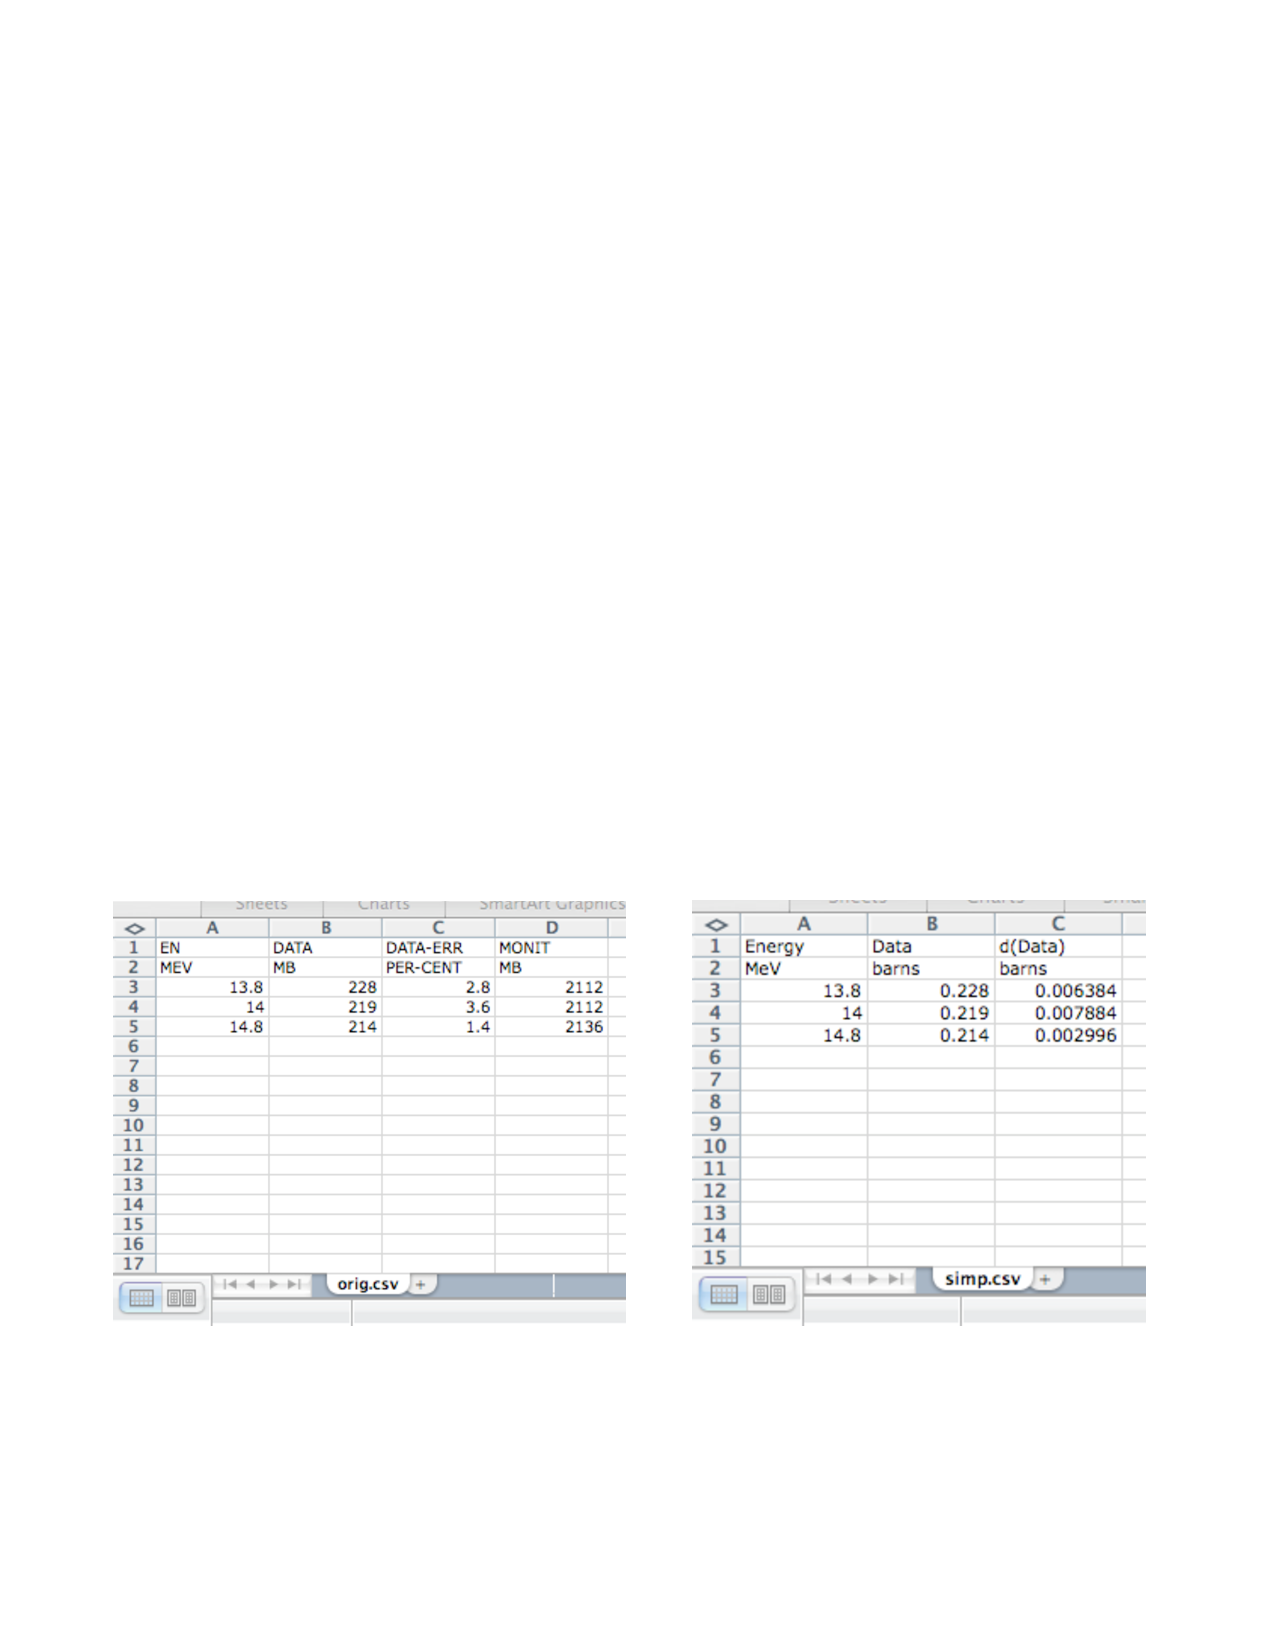
\includegraphics[width=0.9\textwidth]{figs/figure6}
\caption{\label{fig:6}Difference between a ``plain''  \texttt{X4DataSet} (on the left) and a ``simplified'' \texttt{X4DataSet} (on the right).  Note that the units for the simplified set are consistent between a data column and an uncertainty column.  Also notice that cross sections are always given in barns and energies in MeV.  Table \ref{table:columns} lists all the units supported in ``simplified'' \texttt{X4DataSet}s.}
\end{center}
\end{figure}

\begin{table}
\caption{Column names and units in simplified \texttt{X4DataSet}s.}
\begin{center}
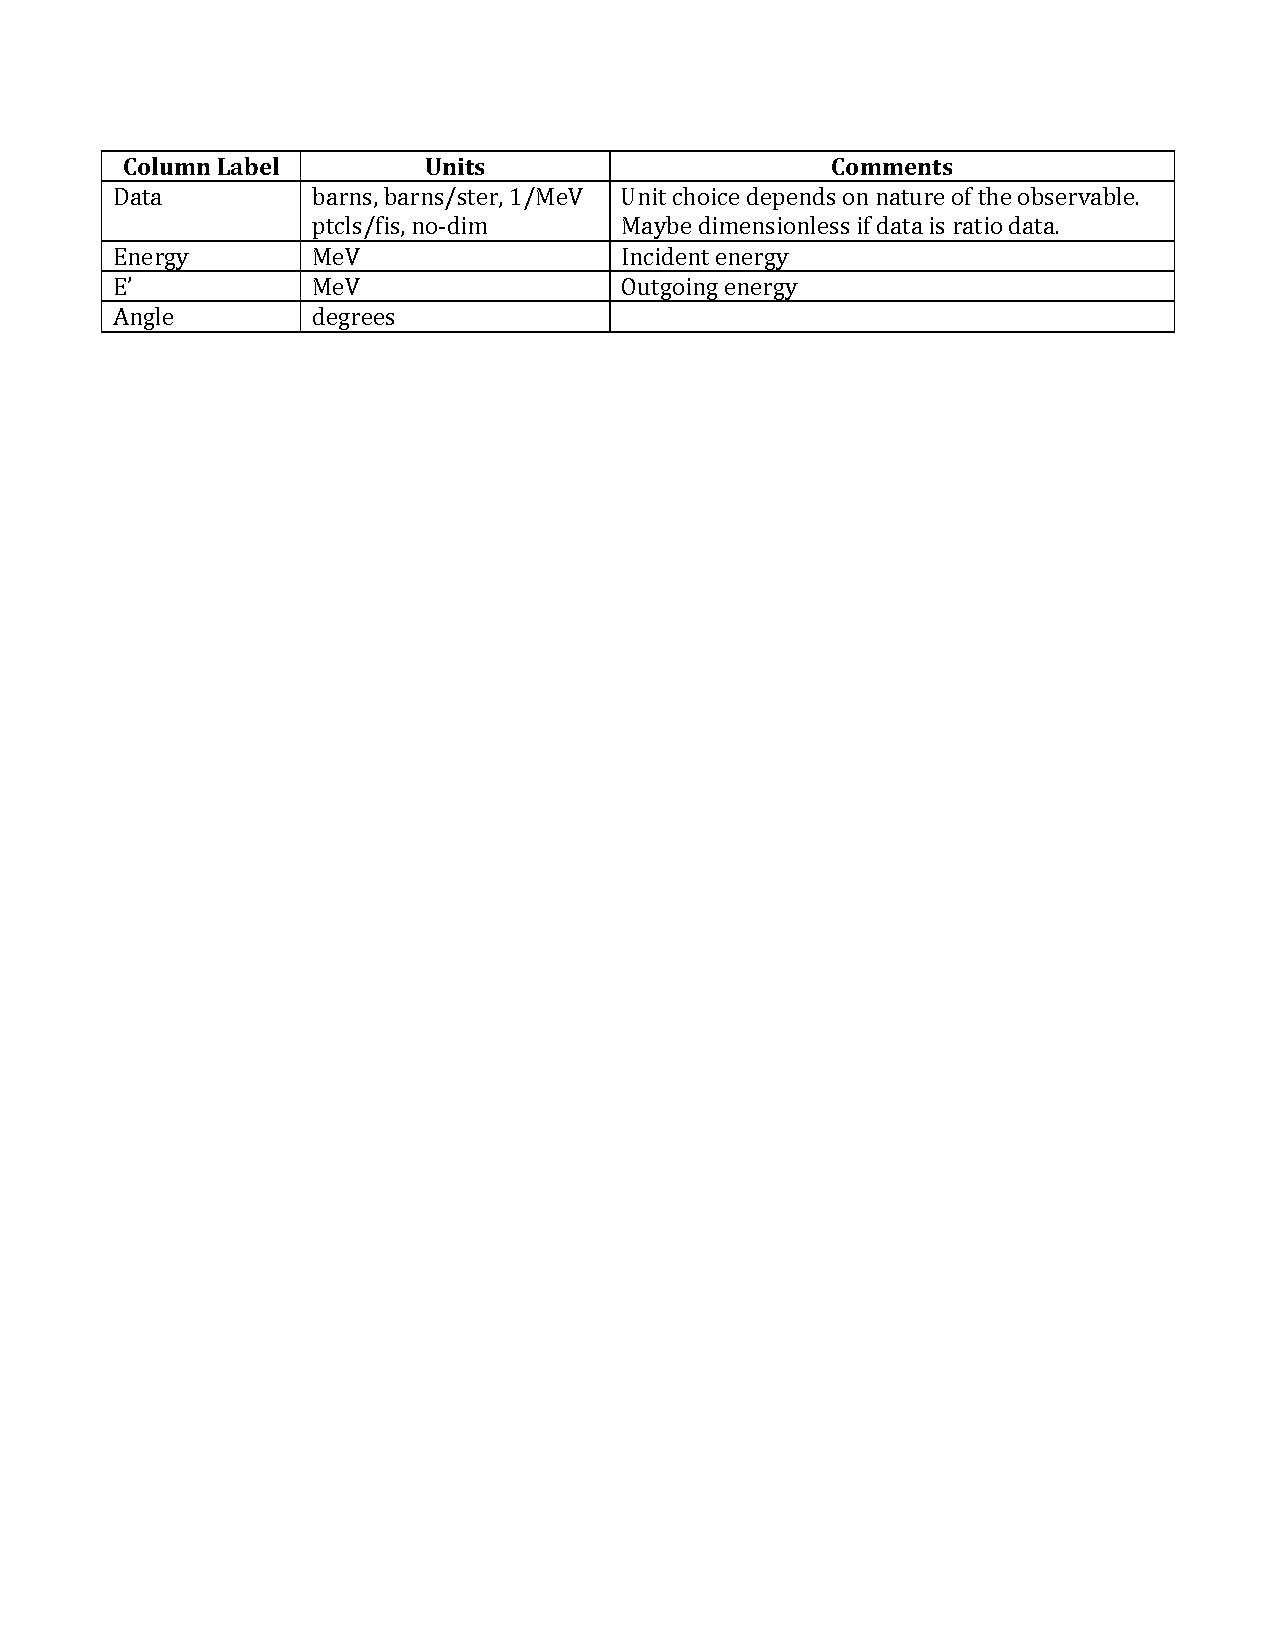
\includegraphics[width=0.9\textwidth]{tables/table4}
\end{center}
\label{table:columns}
\end{table}%

As one can see in Figure \ref{fig:6}, one can think of an \texttt{X4DataSet} as a spreadsheet containing the dataset's values. Indeed, the Python \texttt{\_\_getitem\_\_} operator allows us to directly access elements in this spreadsheet:
\begin{minted}[frame=single,fontsize=\small]{pycon}
>>> dss.keys()
dict_keys([('14129', '14129002', ' ')])
>>> myset = dss[('14129', '14129002', ' ')]
>>> myset['LABELS', 0]
'Energy'
>>> myset['LABELS', 1]
'Data'
>>> myset['UNITS', 1]
'barns'
>>> myset[0, 1]
0.1009
\end{minted}
Of course, \texttt{X4DataSets} also come with meta data describing the set:
\begin{minted}[frame=single,fontsize=\footnotesize]{pycon}
>>> myset.legend()
'(2002) J.A.Becker, L.A.Bernstein, et al.'
>>> myset.citation()
'J.A.Becker, L.A.Bernstein, et al., J.Nucl.Science and Technol.Tokyo,
Supplement 2, (1), 620 (2002);  Data taken from the EXFOR database,
file EXFOR 14129002 dated 2002, retrieved from the IAEA Nuclear Data
Services website.'
\end{minted}
Next, we point out the two methods for exporting the data, the \texttt{csv()} and the \texttt{str()} functions.  The \texttt{csv()} function exports the dataset to a comma separated value file, suitable for viewing in  Microsoft Excel.  The \texttt{str()} function returns a string that can be viewed in the \texttt{xmgrace} plotting package.  The complete list of member functions for the \texttt{X4DataSet} class is given in Table \ref{table:x4dataset}.

Finally, we want to elaborate on the implementation of ``simplified'' \texttt{X4DataSets}.  When the \texttt{getSimplifiedDataSets()} function is called from, it in turn calls the \texttt{getDataSets()} function to get all of the data in an \texttt{X4Entry}.  Then, the \texttt{X4DataSet} function \texttt{getSimplified()} is called to attempt to convert the \texttt{X4DataSet} into its simpler form.  Currently very few quantities in EXFOR can be converted to simpler forms.  The list as of version 1.0 of \xfouri\ is given in Table \ref{table:columns}.


\begin{table}
\caption{Member functions reference for the \texttt{X4DataSet} class and subclasses.}
\begin{center}
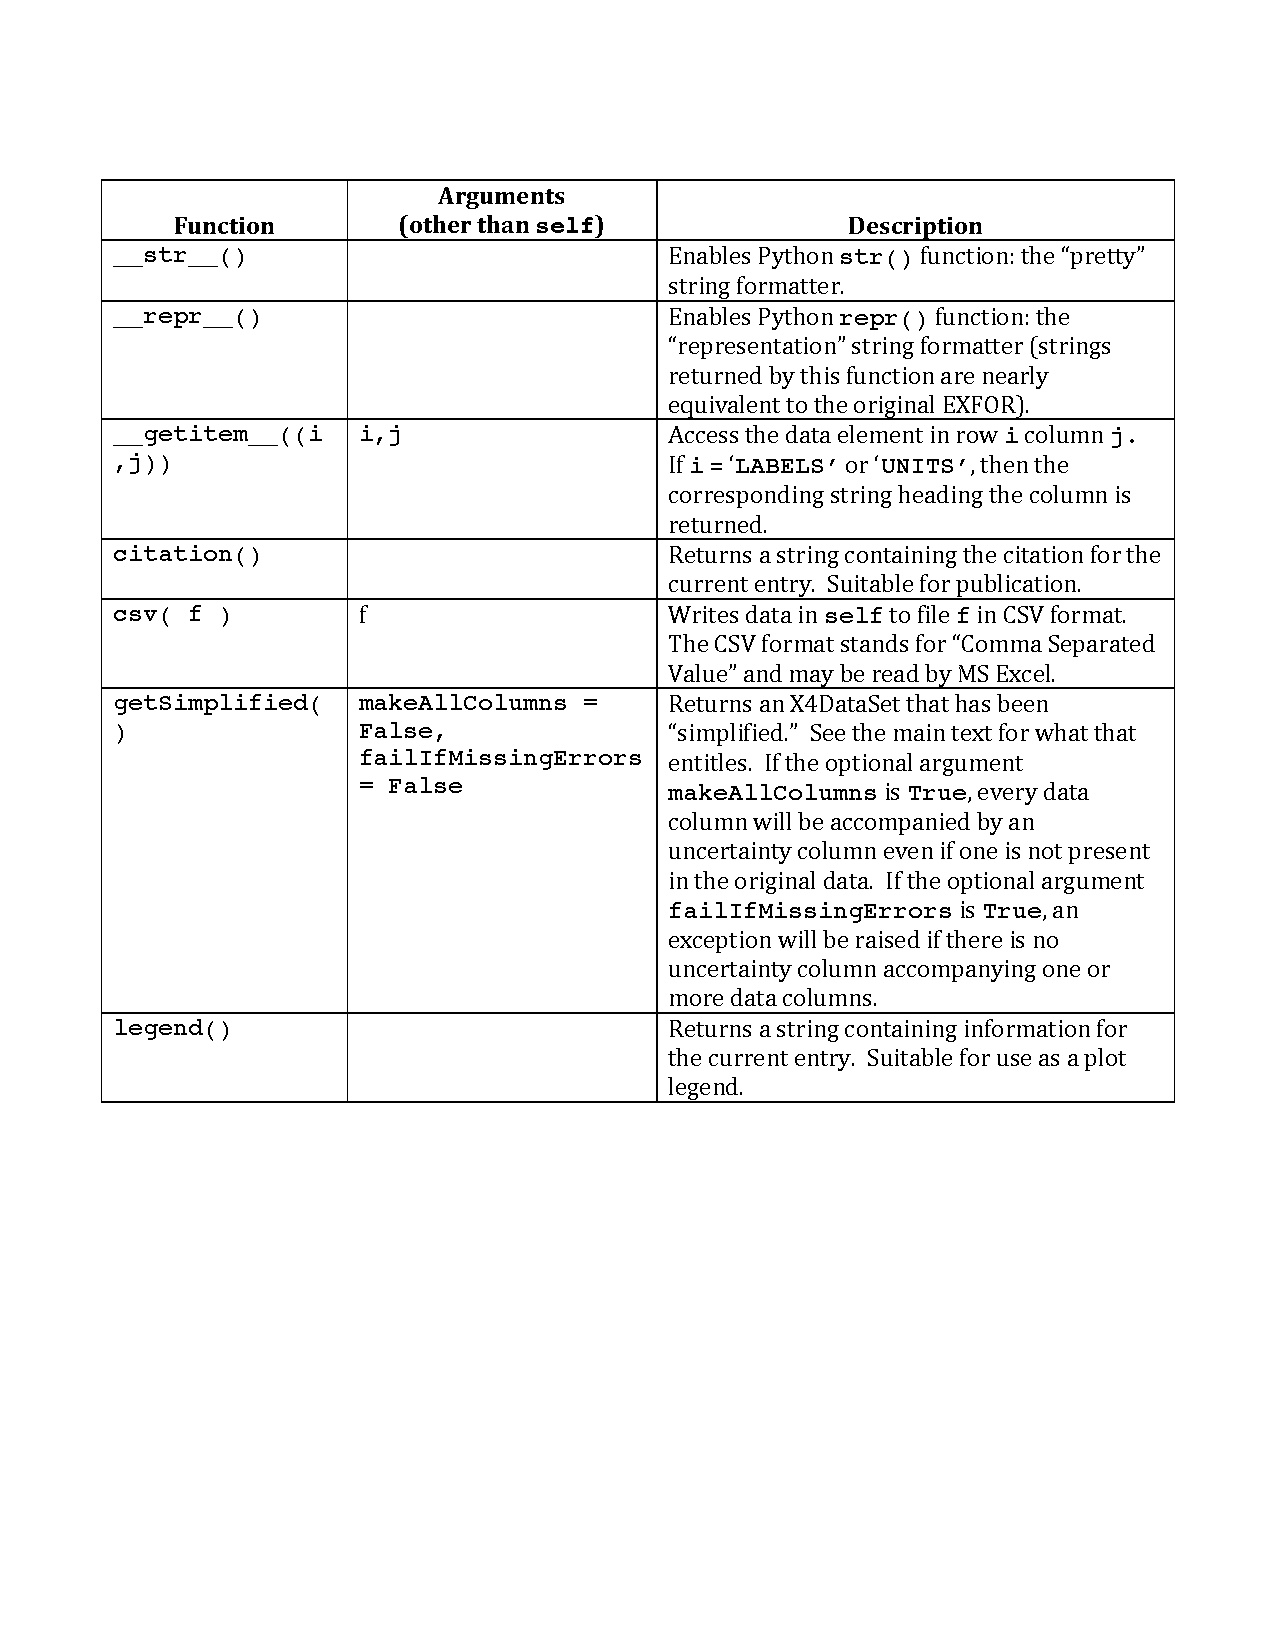
\includegraphics[width=0.9\textwidth]{tables/table5}
\end{center}
\label{table:x4dataset}
\end{table}%

\section{Acknowledgements}
The work at Brookhaven National Laboratory was sponsored by the Office of Nuclear
Physics, Office of Science of the U.S. Department of Energy under Contract No.
DE-AC02-98CH10886 with Brookhaven Science Associates, LLC.
This project was supported in part by the U.S. Department of Energy, Office of Science,
Office of Workforce Development for Teachers and Scientists (WDTS) under the
Science Undergraduate Laboratory Internships Program (SULI).



\addcontentsline{toc}{section}{References}

\thebibliography{99}

\bibitem{web} EXFOR/CSISRS Help page, \url{https://www.nndc.bnl.gov/exfor/compilations/helpX4.html}

\bibitem{1} A. Koning, ``WPEC Subgroup 30: Quality improvement of the EXFOR database Status report  June 2009,'' NEA report number NEA/NSC/WPEC/DOC(2009)416 (2009).

\bibitem{2} O. Schwerer, ``LEXFOR,'' IAEA Nuclear Data Section report number IAEA-NDS-208, Vienna,  Austria (2008).

\bibitem{3} O. Schwerer, ``EXFOR Exchange Formats Manual,'' IAEA Nuclear Data Section report number  IAEA-NDS-207, Vienna, Austria (2008).

\bibitem{4} O. Schwerer, ``EXFOR/CINDA Dictionary Manual,'' IAEA Nuclear Data Section report number IAEA-NDS-213, Vienna, Austria (2008).

\bibitem{5} O. Schwerer, ``EXFOR Basics Manual,''  IAEA Nuclear Data Section report number IAEA-NDS-206, Vienna, Austria (2008).

\end{document}
